\chapter{Obecné informácie o aplikácii}

\section{Motivácia}

Veľmi často v živote narážame na situácie, kedy sa potrebujeme dostať z bodu A do bodu B čo najrýchlejším spôsobom. V mnohých prípadoch mám k dispozícii sieť cestných komunikácii či chodníkov na základe ktorých sa môžeme rozhodovať, ktorá trasa je pre nás vyhovujúca. Pre takéto prípady nám veľmi dobre poslúžia už existujúce navigačné aplikácie ktoré majú podrobne zmapovanú cestnú sieť a vedia nám na základe cestných parametrov určiť najrýchlejšiu alebo najúspornejšiu trasu.

Avšak môžu nastať v živote aj situácie, kedy cestná sieť je priveľmi riedka, až takmer neprítomná. Väčšinou takéto situácie nastávajú vo voľnej prírode, v odľahlých častiach od civilizácie. V takých prípadoch nám konvenčné navigácie veľmi dobre neposlúžia. Ak máme kvalitnú, detailnú mapu, môžeme sa pokúsiť v nej nájsť vyhovujúcu trasu vlastnými silami ale často existuje príliš mnoho možností ktorými sa môžeme vydať. Preto by sa niekedy hodilo mať software, ktorý na základe zadaných parametrov nájde na predloženej mape najrýchlejšiu trasu po ktorej sa človek môže vydať k vytýčenému cieľu.

Príklady využitia takéhoto software-u by sme mohli nájsť v špecifických profesiách ako sú napríklad lesníctvo, záchranné služby či ozbrojené sily. Vo všetkých je potrebné sa z času na čas dostať na miesto ,uprostred ničoho' aby mohli byť vykonané ich zámery.

Takýto software by však našiel uplatnenie taktiež v rekreačných aktivitách. Či už turizmus alebo športové aktivity sa často odohrávajú vo voľnej prírode. Z rôznych dôvodov sa potom môže zísť schopnosť nájdenia najrýchlejšej trasy späť do civilizácie, či už po alebo mimo cesty. 

Rád by som vyzdvihol špecificky jedno športové odvetvie, ktoré veľmi úzko súvisí s hľadaním ciest v otvorenom teréne a to \textit{orientačný beh}. \uv{Orientačný beh (skratka OB) je športové odvetvie vytrvalostného charakteru, pri ktorom je úlohou prejsť alebo prebehnúť podľa mapy a buzoly trať vyznačenú na mape za čo najkratší čas. V teréne nie je trať vyznačená, sú tam umiestnené iba kontrolné stanovišťa (Kontroly)}\cite{CoJeOrientak}. Tento šport bol hlavnou motiváciou pre vytvorenie aplikácie, v ktorej by si užívateľ mohol nechať vykresliť na mape najrýchlejší postup pre ním zadanú trať. 

\section{Aspekty hľadania najrýchlejšej trasy (v OB)}

Mapy pre orientačný beh bývajú veľmi detailné a bežec má preto dostatok informácie na to aby si mohol vybrať ideálnu trasu. Za predpokladu že bežec nerobí chyby a beží presne podľa svojho zámeru, sú pre výber najrýchlejšieho postupu dôležité dva druhy objektov: líniové (cesty, potoky, prieseky, ...) a polygonálne (lúky, kroviská, vodné objekty, močiare, ...). Tie určujú typ terénu nachádzajúci sa v danej časti mapy a tým pádom aj veľkosť odporu ktorý je kladený rýchlosti behu pretekára. Táto veličina sa dá použiť ako hlavný parameter ktorý bude určovať preferencie výberu postupu.

\pagebreak

Proces hľadania cesty sa skladá z dvoch hlavných častí: 
\begin{itemize}
    \item \textbf{vytvorenie mapovej reprezentácie} - Na začiatku je potrené na základe mapového súboru vygenerovať mapovú reprezentáciu na ktorej bude možné vyhľadávať. Mapovou reprezentáciou by mal byť konštrukt, ktorý dobre vystihne topografiu mapy a umožní hľadanie najideálnejšej trasy. V našej aplikácii budú týmito konštruktami \textit{ohodnotené grafy}.  
    \item \textbf{aplikácia vyhľadávacieho algoritmu} - mapová reprezentácia je predaná algoritmu a on za použitia jej interface-u v nej vyhľadá najkratšiu cestu. V našom prípade najkratšia znamená najrýchlejšia.
\end{itemize}

V následujúcich podsekciách spomeniem koncepty, ktoré budú v procese hľadania najrýchlejších ciest vystupovať. Medzi jednotlivými konceptami sú tvorené rozne závislosti. Grafické zhrnutie týchto závislostí je možné nahliadnuť na konci sekcie v Obrázku \ref{obr01:konceptove_zavislosti}.   

\subsection{Mapy}

Na začiatok je potrebné spomenúť koncept Mapy. V procese hľadania ciest bude na viacerých miestach potrebné agregovať dáta z užívateľom vybraného mapového súboru. Aby sme nemuseli neustále čítať priamo zo súboru, budeme si udržovať jeho obsah v pamäti v prívetivejšej forme. 

Touto formou bude práve koncept \textit{Mapy}. Mapa si bude udržovať všetky objekty definované v mapovom súbore a keď bude potrebné agregovať z daného súboru nejakú informáciu (mapovú reprezentáciu, mapovú grafiku, ...) použije sa namiesto súboru odpovedajúci mapový objekt.

Je zahodno zmieniť že koncept mapy je odlišný od konceptu \textit{mapovej reprezentácie}. Mapa narozdiel od jej reprezentácie neobsahuje žiadne zložité prepojenia medzi objektami ktoré v sebe drží. Jej vytvorenie by malo byť rýchle, s lineárnou časovou zložitosťou v závislosti na velkosti mapového súboru.

\subsection{Mapové reprezentácie}

Mapové reprezentácie sú jednou z dôležitých zložiek procesu hľadania ciest. Sú to jednotky, na ktorých sa samotné vyhľadávanie uskutočňuje. Mapové objekty su oproti \textit{mapám} zložitejšie konštrukty ktoré už v sebe zahrňujú plno závislostí a prepojení. Ich generovanie môže zabrať oveľa viac času ako generovanie mapových objektov. 

Ako už bolo spomenuté v aplikácii budú mapovými reprezentáciami \textit{ohodnotené grafy} (naďalej iba grafy). Napriek tomu, že mapová reprezentácia a graf budú v aplikácii reprezentovať rovnaký objekt, ich významy sú odlišné.

\begin{itemize}
    \item \textbf{Mapová reprezentácia} hovorí o tom, ako daný objekt funguje vnútorne. Popisuje jeho vlastnosti, mechanizmy a spôsoby akými generuje výsledný \textit{graf}, v ktorom sa následne hľadá cesta. Objekt ktorý je abstrahovaný z mapy je v prvom rade mapová reprezentácia a až v druhom graf.
    
    Príkladom myšlienky ktorú môže mapová reprezentácia vyjadrovať je \uv{samo-zahusťujúci} sa graf. Takáto mapová reprezentácia počas behu algoritmu zahusťuje predom pripravený graf o ďalšie vrcholy na miestach, v ktorých sa prehľadávanie aktuálne uskutočňuje. Redukuje sa tým veľkosť vygenerovaného grafu.   
    \item\textbf{Graf} na druhej strane hovorí o vlastnostiach objektu ktoré sú viditeľné navonok. Bude informovať o \uv{grafových} službách objektu ktoré dokáže poskytnúť. Tieto služby môžu byť obmedzené práve vnútornou štruktúrou ktorá je definovaná \textit{mapovou reprezentáciou}. Graf sa berie ako druhotný produkt mapového spracovania.   

    Príkladom vlastnosti, ktorú môže graf prezentovať vonkajšiemu svetu je možnosť poskytnutia kompletne vygenerovaného grafu pri ktorom sa vonkajší užívateľ nemusí obávať, že by sa počas práce s ním graf nejakým spôsobom modifikoval. Túto vlastnosť napríklad nevie zaručiť graf ktorý koresponduje s vyššie zmienenou mapovou reprezentáciou ktorá stav grafu počas práce neustále modifikuje, zahusťuje ho.
\end{itemize}

Pojmy \textit{mapová reprezentácia} a \textit{graf} budú naďalej v práci brané ako zameniteľné a ich použitie bude závisieť od okolitého kontextu a ich špecifického významu.

\subsection{Užívateľské modely}

Je potrebné si uvedomiť, že rôzni bežci majú rôzne schopnosti a preto aj ich preferencie na výber trasy nemusia byť rovnaké. Niekto sa dokáže rýchlejšie predierať cez husté pasáže, inému ide rýchlejšie beh cez močiar a ďalšiemu vyhovujú dlhšie postupy po cestách. 

Preto by bolo vhodné, aby užívateľ aplikácie mal možnosť aplikovať svoje preferencie do procesu vyhľadávania. K tomuto účelu boli vytvorené tzv. \uv{užívateľské modely}. Užívateľ si pomocou nich môže vytvoriť vlastný \uv{profil} na základe ktorého bude vyhľadávanie prispôsobené.

Užívateľské modely vďaka svojej informovanosti o užívateľských preferenciách nadobúdajú zodpovednosť za výpočty hodnôt ktoré sú závislé práve na daných preferenciách. Stávajú sa teda dôležitou zložkou procesu hľadania ciest, kde sa vyhľadávacie algoritmy stávajú závislé na nimi vykonávaných výpočtoch.

\subsection{Výškové dáta}

Jedným z dôležitých a neopomenuteľných faktorov voľby najrýchlejšieho postupu je prevýšenie, ktoré je potrebné pri jeho prevedení zdolať. Mnoho typov máp obsahuje popisuje reliéf krajiny pomocou takzvaných \textit{vrstevníc}. Vrstevnica je krivka na mape, ktorá spája body rovnakej nadmorskej výšky. Pre človeka je vrstevnicová abstrakcia výšky terénu veľmi ľahko pochopiteľná a spracovateľná.

Pre strojové spracovanie mapy však vrstevnice predstavujú veľmi neprirodzený spôsob pre reprezentáciu nadmorskej výšky. Vypracovanie reliéfneho obrazu za pomoci vrstevníc samotných je veľmi ťažká úloha. V niektorých prípadoch (mapy pre OB napríklad) dokonca jednotlivé vrstevnice ani nie sú v mapovom súbore reprezentované jedným líniovým objektom. Kvôli dobrej čitateľnosti máp sú často vrstevnice prerušované.
%TODO: mozno najst nejaku tu pracu co sa tym zaoberala, zistit od risa, odkazat na nu

Z vyššie uvedených dôvodov je v aplikácii zahrnutý systém ktorý sprostredkováva užívateľom možnosť stiahnutia a spravovania digitálnych výškových dát ktoré následne môžu byť použité ako pomocný zdroj v procese tvorby mapových reprezentácií. Pre konštrukciu mapových reprezentácií pre niektoré mapové formáty bude nutná prítomnosť zodpovedajúcich výškových dát a pri ich absencii jednoducho nebude možné mapové reprezentácie vytvoriť. 


\subsection{Atribútové template-y}

Ďalšia vec, nad ktorou je potrebné sa zamyslieť je, akým spôsobom sa bude v grafoch mapových reprezentácií uchovávať informácia o mapových vlastnostiach a atribútoch, ktoré konkrétne vrcholy a hrany grafu reprezentujú. Zároveň je potrebné aby dotyčné vlastnosti dokázal príslušný užívateľský model spracovať a dopočítať z nich hodnoty potrebné pre beh vyhľadávacích algoritmov. Používané atribúty, ktoré agregujeme z máp do mapových reprezentácií preto musia byť jednotné v celom procese hľadania cesty, od vytvárania mapovej reprezentácie po samotné spustenie vyhľadávacieho algoritmu.

V aplikácii nám definíciu a jednotnosť atribútov budú zabezpečovať tzv. \textit{template}-y. Každý template bude definovať jedinečnú sadu vrcholových a hranových atribútov. Príkladom pre takúto kolekciu pre potreby OB môže byť napríklad:
\begin{itemize}
    \item vrcholové atribúty - pozícia, výška, indikátory reprezentovaných terénnych objektov (či sa daný vrchol nachádza na ceste, v húštine, na lúke, v dobre priebežnom lese,...)
    \item hranové atribúty - či daná hrana reprezentuje úsek nejakej cesty, hranu nejakého objektu(lúky, húštiny, močiaru,...), sklon terénu
\end{itemize}

Na template-och ako takých bude teda závisieť: 
\begin{itemize}
    \item \textbf{výber užívateľských modelov} - model musí vedieť spracovať atribúty definované daným template-om a vrátiť od neho požadované výsledky.
    \item \textbf{formát vybraného mapového súboru} - musí existovať konvertor mapy špecifického formátu na odpovedajúcu mapovú reprezentáciu, v ktorej vrcholoch a hranách sú obsiahnuté atribúty definované daným template-om. Túto závislosť môžeme brať aj opačným smerom. Pre vybraný mapový formát môžeme zvoliť len použiteľný template.
\end{itemize}

\subsection{Vyhľadávacie algoritmy}

Nakoniec nemôžeme opomenúť koncept samotných vyhľadávacích algoritmov, poslednú neodmysliteľnú súčasť procesu hľadania ciest. Vyhľadávací algoritmus, podobne ako \textit{mapová reprezentácia}, reprezentuje koncept vnútorného mechanizmu ktorým je najkratšia cesta v grafe hľadaná. Príkladom takéhoto algoritmu môže byť napríklad algoritmus \textit{A*}. 

Vstupom do každého algoritmu sú:
\begin{itemize}
    \item \textbf{graf}, na ktorom je hľadanie najkratšej cesty vykonané a 
    \item \textbf{užívateľský model}, ktorý algoritmus nutne potrebuje ku výpočtom váh grafových hrán a iných hodnôt potrebných k jeho správnemu chodu.  
\end{itemize}
  
Každý algoritmus následne ponúka množinu jeho implementácií. Každá implementácia definuje množinu vlastností, ktoré vložený graf a užívateľský model musia spĺňať. Napríklad implementácie A* algoritmu budú požadovať, aby užívateľský model bol schopný, popri výpočte váh pre hrany grafu, dodať ešte aj výpočet heuristiky využívanej v tomto algoritme.


\begin{figure}[h]\centering
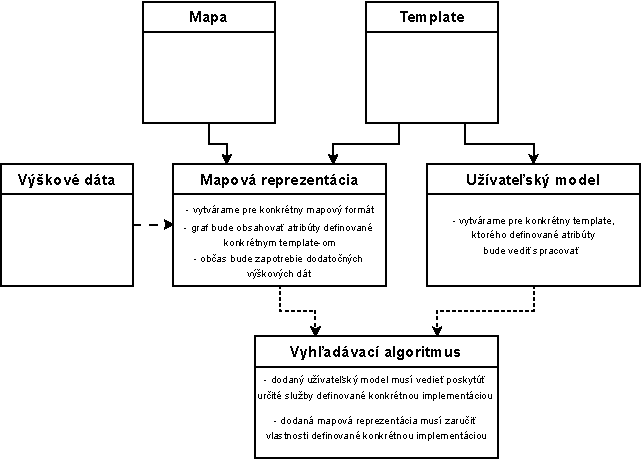
\includegraphics[]{img/konceptove_zavislosti}
\caption{Diagram závislostí jednotlivých konceptov} 
\label{obr01:konceptove_zavislosti}
\end{figure}

\pagebreak

\section{Zvolené prostriedky}

\subsection{Použitý programovací jazyk}

Pre implementáciu aplikácie bol vybraný jazyk C\#. Jazyk bol vybraný pre jeho jednoduchosť a bezpečnosť použitia. Alternatívnou volbou by mohol byť jazyk Java, ktorý má blízko práve ku C\#. Jeho nedostatočná znalosť v dobe začiatku práce ho však vyradila z použiteľných možností. 

Ďalšími možnosťami by mohol byť buď typicky vysoko-úrovňový jazyk Python alebo na druhú stranu nízko úrovňový jazyk C++. Nakoľko v aplikácii bude prebiehať mnoho výpočtov, python by nebol vhodnou voľbou pre nedostatočnú rýchlosť z neho vytvoreného strojového kódu. Na druhú stranu C++ by bol veľmi dobrým kandidátom z hladiska výpočtovej sily. V tomto prípade však narážame opäť na nie veľmi dobrú znalosť tohto jazyka a na nie úplne pohodlnú prácu s ním. Pri takomto väčšom projekte sme považovali za potrebné istotu, že nás použitý jazyk podrží (ak s ním nie sme zžitý na 100\%). 

Vhodnou úpravou by možno bolo implementovať výpočtovo náročné procesy v jazyku typu C++ a následne túto implementáciu volať externe z C\# jadra.     

\subsection{Užívateľské rozhranie}

Pre implementáciu užívateľského rozhrania som sa rozhodol pre \textit{Avalonia UI} framework. 

V C\# existuje viacero možných framework-ov z ktorých bolo možné si vybrať:
\begin{itemize}
    \item GUI knižnice, ktoré sú súčasťou samotného .NET framework-u:
    \begin{itemize}
        \item \textbf{Windows Forms} je klasická GUI knižnica. Je jednoducho použiteľná a vďaka jej dlhoročnej podpore aj robustná a spoľahlivá. Jej vek je však aj jej nevýhodou, nakoľko vzhľad aplikácií vytvorených za pomoci Windows Forms príde človeku pomerne zastaralý. Ďalšou nevýhodou je rastrová povaha jeho renderovcieho engine-u. Táto vlastnosť sa nehodí pre aplikáciu, ktorej jedným z hlavných účelov je vykreslovanie mapových, vektorových objektov.     
        \item \textbf{Windows Presentation Foundation (WPF)} je modernejší nástupca Windows Forms. Aplikácie tvorené touto knižnicou majú modernejší vzhľad, sú generované renderovacím enginom založeným na vektorovej grafike. Ku programovaniu sa tu využíva popri C\# aj XAML v ktorom sa definuje layout užívateľského rozhrania. Avšak spoločne s Windows Forms je ich spoločnou nevýhodou platformová závislosť na operačnom systéme Windows.
        \item \textbf{.NET MAUI} je nástupcom \textit{Xamarin.Forms}. Je to open-source-ový cross-platformný framework s množinou UI nástrojových balíčkov pre jednotlivé platformy. Podobne ako vo WPF sa pre vytváranie UI využíva kombinácia C\# a XAML. 
    \end{itemize}
    \item Alternatívou ku vstavaným .NET GUI knižniciam je práve nezávislá, open-source knižnica \textbf{Avalonia UI}. Čo do vlastností je veľmi dobre porovnateľná s \textit{.NET MAUI}. Hlavný rozdiel medzi týmito dvomi knižnicami je v~spôsobe, akým vykresľujú užívateľské rozhranie. Avalonia zapojuje kresliaci engine poháňaný knižnicou pre 2D grafiku \textit{Skia}. Na druhú stranu MAUI využíva natívne nástrojové balíčky pre každú platformu. Ďalším rozdielom je, že Avalonia, na rozdiel od MAUI, podporuje aj niektoré distribúcie Linuxových systémov.
\end{itemize}

Rozhodnutie nakoniec padlo na využitie framework-u Avalonia UI. Nakoľko je veľmi podobný natívnemu .NET MAUI, rozhodla podpora pre Linuxové systémy a aj kvalitne spravená dokumentácia, z ktorej sa ľahko dalo pochopiť, ako sa s knižnicou má pracovať. 

Informované rozhodnutie pre výber GUI knižnice bolo učinené na základe zdrojov \cite{WpfGuide,WhatIsMAUI,AvaloniaMauiComparison}. Zároveň väčšinu informácií, ktoré som o Avalonia UI počas tvorby programu čerpal pochádzali z jej dokumentácie \cite{AvaloniaDokumentacia}.

\subsection{Architektúra Model-View-ViewModel (MVVM)}\label{ArchitekturaMVVM}

Jeden z ďalších dôležitých aspektov ktorý hral dôležitú úlohu vo výbere knižnice pre užívateľské rozhranie bola podpora MVVM návrhového vzoru. Dokumentácia Avalonia UI popisuje architektúru MVVM následovne: \uv{The Model-View-View Model (MVVM) pattern is a common way of structuring a UI application. It uses a data binding system that helps move data between its view and view model parts. This means it achieves separation of application logic (view model) from the display of the UI (view). Separation between the application logic and the business services (model) is commonly achieved by a Dependency Injection (DI) system.}\cite{MVVMDefByAvalonia}.

MVVM architektúra je vhodná pre našu aplikáciu, nakoľko pre jej rozsah by klasická \textit{event-driven code-behind} architektúra nemusela postačovať. Týmto spôsobom zaručíme lepšiu separáciu a dostačujúcu vnútornú nezávislosť kódu.    

V našej aplikácii bude tento návrhový vzor uplatnený s jemnou obmenou. Vrstva view model, ktorá v pôvodnom návrhovom vzore zastávala úlohu logiky aplikácie bude rozdelená na dve časti: view model a novo vzniknutý \textit{model view}. Viac informácií o tejto úprave je možné nájsť v sekcii \ref{MVVMNavrhovyVzor}. 

\subsection{Reaktívne programovanie}

Ďalším dôležitým aspektom v aplikácii je Avaloniou a architektúrou MVVM iniciované využitie \textit{reaktívneho programovania.} Avalonia pre aplikáciu tohto paradigma využíva framework \textbf{Reactive UI}. 

Tá samotná definuje reaktívne programovanie ako \uv{Reactive programming is programming with asynchronous data streams.} a dodáva \uv{Event buses or your typical click events are really an asynchronous event stream, on which you can observe and do some side effects. Reactive programming is that idea on steroids. You are able to create data streams of anything, not just from click and hover events. Streams are cheap and ubiquitous and anything can be a stream: variables, user inputs, properties, caches, data structures, etc.}\cite{ReactiveProgrammingByReactiveUI}.

V aplikácii sa bude tento framework využívať prevažne vo vrstvách view a view model. Vrstvy model view a model sa väčšinou zaobídu bez jeho využitia, nakoľko reaktívna komunikácia prebieha medzi vrstvami view a view model.   